\chapter{About the Template}
%\label{chapter:title}

This template aims to simplify and improve the (Xe)LaTeX report template by Delft University of Technology. Some of the main features:

\begin{itemize}
  \item \textbf{Simplicity First:} A class file that has been reduced by nearly 70\% to simplify customization;
  \item \textbf{Effortless:} A careful selection of common packages to get started immediately;
  \item \textbf{Complete:} Ready-to-go when it comes to the document and file structure.
\end{itemize}

\noindent This template works with pdfLaTeX, XeLaTeX and LuaLaTeX. In order to adhere to the TU Delft house style, either XeLaTeX or LuaLaTeX is required, as it supports TrueType and OpenType fonts. BibLaTeX is used for the bibliography with as backend biber. Please visit \url{https://dzwaneveld.github.io/report} for the full documentation.

\begin{figure}[h]
    \centering
    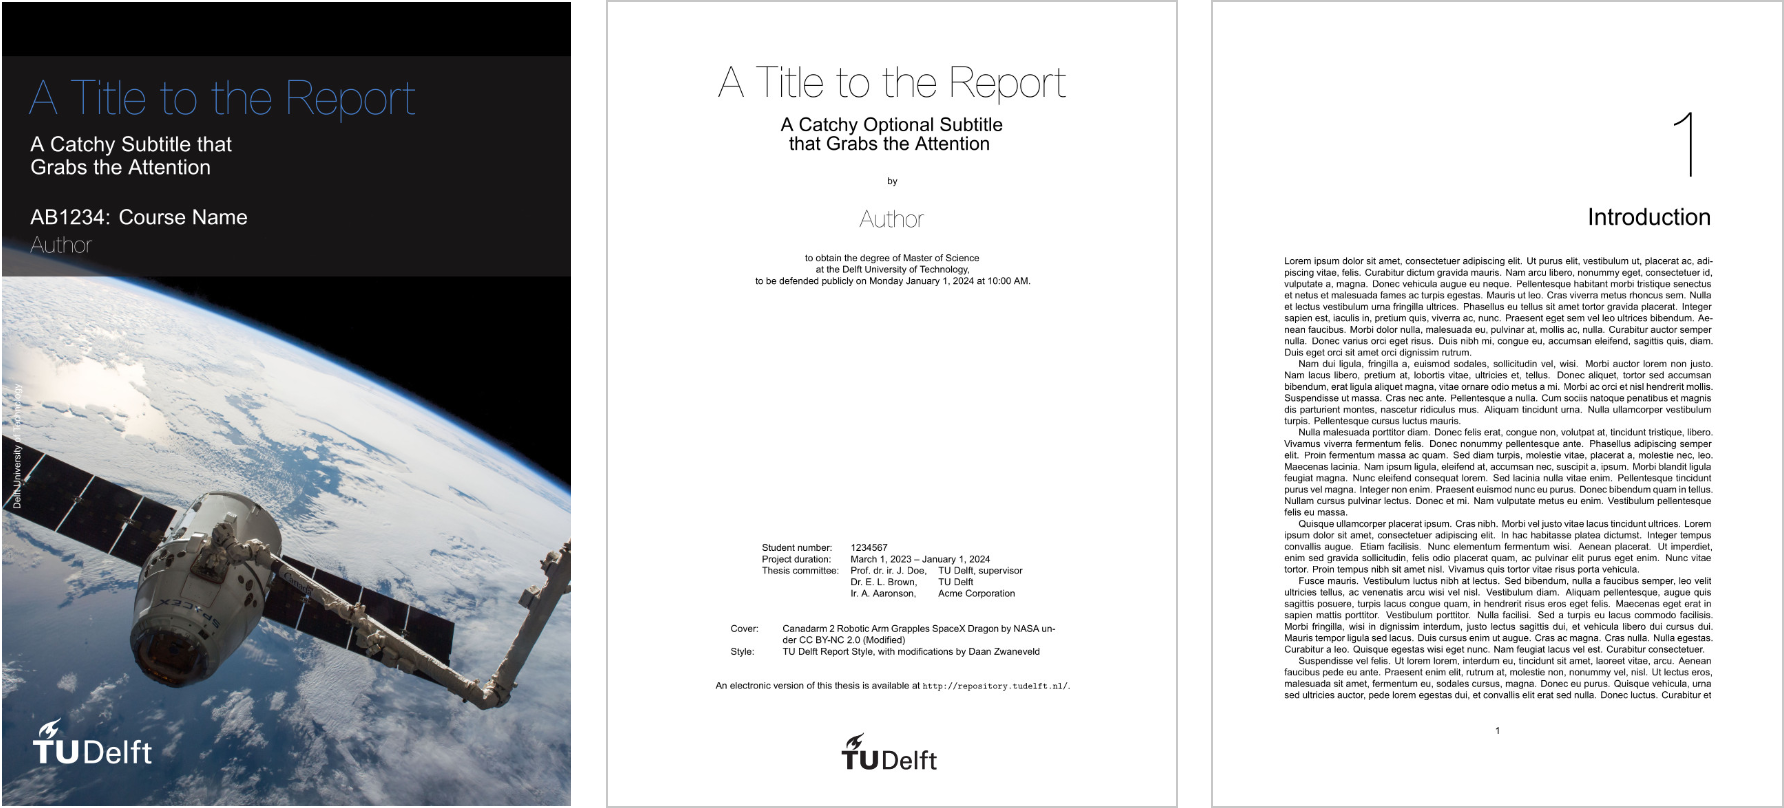
\includegraphics[width=0.95\linewidth]{figures/template.png}
    \caption{Preview of the template}
\end{figure}

\section*{License}

This template by Daan Zwaneveld is licensed under CC BY-NC 4.0. To view a copy of this license, visit \url{https://creativecommons.org/licenses/by-nc/4.0/}. No attribution is required in PDF outputs created using this template.
